\documentclass[tikz,border=4pt]{standalone}
\usepackage{amsmath}
\usepackage{tikz}
\usetikzlibrary{shapes.geometric, arrows.meta, positioning}

\begin{document}
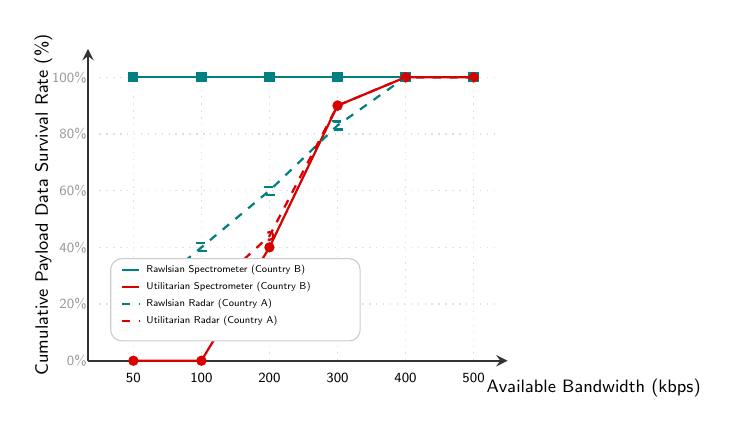
\begin{tikzpicture}[
    scale=0.72,
    transform shape,
    font=\sffamily\small,
    axis/.style={thick, ->, >=stealth, draw=black!80},
    grid/.style={draw=gray!25, dotted, line width=0.5pt},
    labelstyle/.style={font=\sffamily\scriptsize}
]
    % Grid lines (Y-axis grid)
    \foreach \y/\pct in {0/0\%, 1/20\%, 2/40\%, 3/60\%, 4/80\%, 5/100\%} {
        \draw [grid] (0.0, \y) -- (7.0, \y);
        \node [left, font=\scriptsize\sffamily, text=gray!80] at (-0.1, \y) {\pct};
    }
    
    % Grid lines (X-axis grid)
    \foreach \x/\val in {0.6/50, 1.8/100, 3.0/200, 4.2/300, 5.4/400, 6.6/500} {
        \draw [grid] (\x, 0) -- (\x, 5.2);
        \node [below, font=\scriptsize\sffamily] at (\x, -0.1) {\val};
    }
    
    % Axes
    \draw [axis] (-0.2, 0) -- (7.2, 0) node [below right, xshift=-0.5cm, yshift=-0.2cm] {Available Bandwidth (kbps)};
    \draw [axis] (-0.2, 0) -- (-0.2, 5.5) node [midway, above, rotate=90, yshift=0.5cm] {Cumulative Payload Data Survival Rate (\%)};
    
    % Data Lines
    % 1. Rawlsian Spectrometer (Solid Teal with Squares)
    \draw [thick, teal, mark=square*, mark options={fill=teal}] plot coordinates {
        (0.6, 5.0) (1.8, 5.0) (3.0, 5.0) (4.2, 5.0) (5.4, 5.0) (6.6, 5.0)
    };
    
    % 2. Utilitarian Spectrometer (Solid Red with Circles)
    \draw [thick, red!85!black, mark=*] plot coordinates {
        (0.6, 0.0) (1.8, 0.0) (3.0, 2.0) (4.2, 4.5) (5.4, 5.0) (6.6, 5.0)
    };
    
    % 3. Rawlsian Radar (Dashed Teal with Open Squares)
    \draw [thick, dashed, teal, mark=square] plot coordinates {
        (0.6, 1.0) (1.8, 2.0) (3.0, 3.0) (4.2, 4.15) (5.4, 5.0) (6.6, 5.0)
    };
    
    % 4. Utilitarian Radar (Dashed Red with Open Circles)
    \draw [thick, dashed, red!85!black, mark=o] plot coordinates {
        (0.6, 0.55) (1.8, 1.1) (3.0, 2.2) (4.2, 4.5) (5.4, 5.0) (6.6, 5.0)
    };
    
    % Custom TikZ Legend (Guaranteed Compile Proof)
    \begin{scope}[shift={(0.2, 0.35)}]
        \draw [draw=black!20, fill=white, rounded corners] (0, 0) rectangle (4.4, 1.45);
        
        \draw [thick, teal, mark=square*, mark options={fill=teal}] (0.2, 1.25) -- (0.5, 1.25) node [right, font=\tiny\sffamily, text=black] {Rawlsian Spectrometer (Country B)};
        \draw [thick, red!85!black, mark=*] (0.2, 0.95) -- (0.5, 0.95) node [right, font=\tiny\sffamily, text=black] {Utilitarian Spectrometer (Country B)};
        \draw [thick, dashed, teal, mark=square] (0.2, 0.65) -- (0.5, 0.65) node [right, font=\tiny\sffamily, text=black] {Rawlsian Radar (Country A)};
        \draw [thick, dashed, red!85!black, mark=o] (0.2, 0.35) -- (0.5, 0.35) node [right, font=\tiny\sffamily, text=black] {Utilitarian Radar (Country A)};
    \end{scope}
    
\end{tikzpicture}
\end{document}
